%!TEX root = P231_notes.tex
%% From: 2917 Lec 22 and onward
\section{Nuts and Bolts Probability}
\label{sec:probability}

Let's forget Green's functions now and follow up on something to do with probability: Bayes' theorem. This is fully outside the scope of the class, but it is significant enough that it deserves to be mentioned in a `math methods' course. 

You are already familiar with \emph{conditional probability}. If you roll two 6-sided dice, the probability of each coming up with one is simply the product of each probability:
\begin{align}
	P(\text{both dice are 1}) = P(\text{one die is 1})^2 \ .
\end{align}
In this case we're asking about two events, $A$ (first die rolls 1) and $B$ (second die rolls 1). In general, though, these two events may not be independent. In this case, one has to deal with \emph{conditional probability}. We write $P(A|B)$ to mean the probability of $A$ assuming that $B$ is true. This, in turn, is related to the probability that $A$ \emph{and} $B$ are true divided by the probability that $B$ is true:
\begin{align}
	P(A|B) &= \frac{P(A\& B)}{P(B)} \ .
	\label{eq:P:A:given:B}
\end{align}
Stop to make sure this makes sense: if you write the probabilities as
\begin{align}
	P(X) = \frac{\text{number of times $X$ happens}}{\text{total number of samples}} \ ,
\end{align}
then the right-hand side of \eqref{eq:P:A:given:B} is simply
\begin{align}
	P(A|B) = \frac{\text{number of times $A$ and $B$ happen}}{\text{number of times $B$ happens}} \ , 
\end{align}
which is precisely what we want from $P(A|B)$: what is the probability that $A$ is true if we already know $B$ is true. Once we say $B$ is true, we can throw away all the samples where $B$ is not true.

Here's the key insight: $P(A|B)P(B) = P(A\& B)$. On the right hand side, $A\&B$ is completely symmetric in $A$ and $B$. That means we could swap them on the left-hand side as well: 
\begin{align}
	P(A\&B) = P(B\& A) = P(B|A)P(A) \ . 
\end{align}
We thus have $P(A|B)P(B)=P(B|A)P(A)$, which gives us the famous \textbf{Bayes theorem} that relates the conditional probabilities $P(A|B)$ and $P(B|A)$:
\begin{align}
	P(A|B) &= \frac{P(B|A) P(A)}{P(B)} \ .
\end{align}
Here's a useful graphical representation from Bob Cousins:
\begin{center}
\includegraphics[width=.8\textwidth]{figures/ConditionalProb.png}
\end{center}
What is important here is that $P(A|B)$ and $P(B|A)$ can differ significantly if $P(A)/P(B)$ is very big or very small. This can be problematic because human beings can be sloppy when distinguishing $A|B$ versus $B|A$. 
\begin{example}
The probability that someone knows how to use \texttt{ROOT}\footnote{\url{https://root.cern/}} given that they are a particle physicist is roughly $P(\text{\texttt{ROOT}}|\text{particle person}) \approx 50\%$. To rough approximation, particle experimentalists use \texttt{ROOT} and theorists avoid it like the plague. However, the probability that someone is a particle physicist given that they use \texttt{ROOT} is $P(\text{particle person}|\text{\texttt{ROOT}}) \approx 100\%$. If someone uses \texttt{ROOT}, then you can be pretty sure that they do particle physics.
\end{example}

There's a simple reason why this is important: usually $A$ is something that we can actually see and $B$ is something that we want to \emph{infer} but cannot directly test. Specifically, in physics we typically have the following case:
\begin{align}
	A &= \text{data} 
	&
	B &= \text{theory} \ .
\end{align}
$A$ is the particular data that an experimentalist or an observer actually records. $B$ roughly a statement about whether a theory is correct. 
% 
We've already made may caveats in Section~\ref{sec:EFT:philosophy} about the idea of effective theories and what it means for a theory to be `correct.' To summarize, usually $B$ is asking: is a given theory a good description of the underlying phenomenon related to the data $A$? 

At this point, I'll leave it to you to dig deeper into the formalism for probabilities\footnote{Some of my favorite references: \emph{Statistics: A Guide to the Use of Statistical Methods in the Physical Sciences}, the lectures by Bob Cousins \texttt{1807.05996} (and his 1995 \emph{American Journal of Physics} article), and Kyle Cranmer's statistics and data science textbook~\url{https://cranmer.github.io/stats-ds-book/}.}. In summary, you should be precise about your hypothesis tests and be able to clearly articulate the meaning of whatever figure of merit you're using to interpret your data. In what follows, let's just play with some silly manifestation of these ideas. 

\subsection{Were we lucky that the LHC didn't destroy the world?}
\label{sec:LHC:luck}

One of the favorite discussion topics when I was a graduate student was a funny clip from \emph{The Daily Show} about the Large Hadron Collider in 2009\footnote{\url{http://www.cc.com/video-clips/hzqmb9/the-daily-show-with-jon-stewart-large-hadron-collider}}
. At the time, there was speculation that the LHC could destroy the world. There were many fun and silly ideas for how this could come about, though there were many very good reasons why these ideas were more `silly science fiction' rather than environmental concern\footnote{\url{https://home.cern/science/accelerators/large-hadron-collider/safety-lhc}}. During the clip, John Oliver---then a correspondent for John Stewart's \emph{The Daily Show}---interviews some dude concerned about the possibility that the \acro{LHC} may destroy the world. The interview went something like this:
\begin{quote}
\textsc{Oliver}: What are the chances that the world is going to be destroyed?\\
\textsc{Dude}: It's about a one in two chance.\\
\textsc{Oliver}: 50--50?\\
\textsc{Dude}: It's either going to happen or not happen. So the best guess is 50--50.
\end{quote}
\begin{exercise}
What's wrong with that dude's argument?
\end{exercise}
 

\subsection{The Prosecutor's Fallacy}


This comes from Bergstrom and West's book \emph{Calling Bullshit}. Imagine some high-profile \emph{Ocean's Eleven} or \emph{Carmen Sandiego} style heist. The \acro{FBI} is able to recover a set of fingerprints which they run through their database of 50 million people and guess what: \emph{you're} a match. Against everyone's advice, you decide to represent yourself in court. When the \acro{FBI} agent explains that your fingerprint match makes is an open-and-shut case, you politely ask: \emph{what is the chance that the wrong fingerprint would be matched with a print in the database?}

``Hah!'' the prosecutor scoffs at you. ``The chance of this happening happens to be \emph{one in ten million}. That's beyond any reasonable doubt.'' Fortunately you know a thing or two about probability and there's a chalkboard in the courtroom. You draw the following table:
\begin{center}
\begin{tabular}{l|ll} \toprule % @{} removes space
		& Match & No Match
		\\ \hline
		Guilty & \phantom{1 person} & \phantom{0 people}
		\\
		Innocent & \phantom{5 person} & \phantom{50,000,000 people}
		\\ \bottomrule
\end{tabular}
\end{center}
You start by stating the obvious assumptions. There is \emph{one} guilty person---not you---whose fingerprints match the prints lifted from the crime scene. While it's neither here nor there, you also point out that there are no people who are both guilty but whose prints do not match those at the crime scene. You start to fill in the table:
\begin{center}
\begin{tabular}{l|ll} \toprule % @{} removes space
		& Match & No Match
		\\ \hline
		Guilty & {1 person} & {0 people}
		\\
		Innocent & \phantom{5 person} & \phantom{50,000,000 people}
		\\ \bottomrule
\end{tabular}
\end{center}
Next you say that there are approximately 50 million people in the fingerprint database. Almost all of theme are innocent and almost all of them are completely distinct from the evidence from the crime scene. You fill in the table a bit more:
\begin{center}
\begin{tabular}{l|ll} \toprule % @{} removes space
		& Match & No Match
		\\ \hline
		Guilty & {1 person} & {0 people}
		\\
		Innocent & \phantom{5 person} & {50,000,000 people}
		\\ \bottomrule
\end{tabular}
\end{center}
Finally, you point out: given a false-match rate of one in 10 million, you can estimate that around \emph{five} innocent people will have fingerprints that match those at the crime scene. 
\begin{center}
\begin{tabular}{l|ll} \toprule % @{} removes space
		& Match & No Match
		\\ \hline
		Guilty & {1 person} & {0 people}
		\\
		Innocent & {5 person} & {50,000,000 people}
		\\ \bottomrule
\end{tabular}
\end{center}
The prosecutor starts to sweat, they can see what's coming. You point out that the \emph{data} in the case is that you are one person whose fingerprints match those at the crime scene. That means we should focus only on the population of people whose fingerprints match those the crime scene: there are approximately six: five innocent and one guilty. You point to the numbers and say, ``I know that my \emph{Math Methods} class in graduate school wasn't \emph{especially} rigorous, but clearly there is a five in six chance that even though my fingerprint matches the one from the crime scene, I am in fact innocent.''
\begin{exercise}
What was the mistake that the prosecutor made?
\end{exercise}
Bergstrom and West made up the above story to explain the fallacy, but they point out that this scenario indeed played out in 2018 in the highly publicized case that led to the capture of the Golden State Killer using \acro{DNA} samples from a genealogy company. What was not shared widely in the press coverage was that the genetic screening alone initially led to the \emph{wrong} suspect. The true culprit was identified by combining the \acro{DNA} match with other evidence from more traditional detective work. Timely applications to medicine are all over\footnote{\url{https://youtu.be/lG4VkPoG3ko}}.

\subsection{Why we are not evidence for God}

Mathematician Jordan Ellenberg takes the above example a bit further to highlight another fallacy. This comes from his pop mathematics book \emph{How Not To Be Wrong}, which you're probably a bit advanced for, but is none-the-less a fun read and a lesson in effective technical communication to a lay audience. 

There is an argument that the universe we observe is evidence for God. After all, look how incredibly engineered and fine-tuned life is\footnote{You can also point to more physical arguments, like the apparent fine tuning of the cosmological constant.}. Indeed all this \emph{stuff} that we see around us does seem rather complicated---why isn't the universe more like the spherical cow\footnote{\url{https://en.wikipedia.org/wiki/Spherical_cow}} theories that we study in grad school? 

The argument is something like the one in Appendix~\ref{sec:LHC:luck}. Let's write down the \emph{likelihood} that we see this complicated universe. Ellenberg makes some very rough estimates that will be sufficient for our point. The existence of an omnipotent creator could seems to be far more likely to have created such a finely-tuned, complicated universe.
\begin{center}
\begin{tabular}{l|ll} \toprule % @{} removes space
		& God Exists & No God
		\\ \hline
		Simple universe &  & 
		\\
		Complicated universe & $10^{-6}$  & $10^{-18}$
		\\ \bottomrule
\end{tabular}
\end{center}
We don't bother to write out the first row---after all, that's not the case we care about. There you have it: it seems like the observation that our universe is complicated gives overwhelming evidence that God exists. 

Of course, the problem is that we have \emph{assumed} that God exists and God doesn't exist are the only possible outcomes. This is analogous to assuming that you have a theory for an exotic new particle and the results of an experiment either rejects existence of the exotic new particle in favor of the null hypothesis (no new particles) or confirms the existence of the exotic new particle (alternate hypothesis). You know this is too na\"ive. Sometimes there are other reasons why the data of your experiment looks funny---maybe you didn't plug in your cables properly\footnote{\url{https://en.wikipedia.org/wiki/Faster-than-light_neutrino_anomaly}}. So in our ontological argument, Ellenberg says that we should be sure to consider all possibilities. For example, often times complicated things come about by the dreaded `design by committee.' So maybe it's not that God exists, but that there's a whole pantheon of gods who designed the universe through a complex process of peer review and feedback. The result is \emph{this} ugly mess. Our table now looks like
\begin{center}
\begin{tabular}{l|lll} \toprule % @{} removes space
		& God Exists & No God & Many Gods
		\\ \hline
		Simple universe &  & &
		\\
		Complicated universe & $10^{-6}$  & $10^{-18}$ & $10^{-5}$
		\\ \bottomrule
\end{tabular}
\end{center}
The number we threw in here is fairly arbitrary, but the point is that you could make the argument that \emph{many gods} may be more likely than \emph{one god}. Fine, but for a physics class this is starting to look a little bit too much like religious studies, no? Well, as we ponder the origin of our universe, we go to knock on the door of our cosmology colleagues, only to find that they're busy running their cosmological simulation. Aha! You remember playing \emph{The Sims}, which is an odd knock-off experience compared to actual real life. However, it seems plausible that a sufficiently advanced civilization would have created a computer game to simulate their existence. Perhaps when that simulated reality is sufficiently advanced, it too will create a computer program that simulates \emph{their} reality. And so forth. You start to think that this, too, is a rather plausible origin for a strangely complicated universe. Ellenberg updates our table as follows
\begin{center}
\begin{tabular}{l|llll} \toprule % @{} removes space
		& God Exists & No God & Many Gods & Simulated reality
		\\ \hline
		Simple universe &  & & &
		\\
		Complicated universe & $10^{-6}$  & $10^{-18}$ & $10^{-5}$ & $10^{-1}$
		\\ \bottomrule
\end{tabular}
\end{center}
At the level of this crude example, it seems that the most likely possibility is that not only does any god \emph{not} exist, but it's unlikely that we exist. 

\subsection{The End of the World}

There's a cute example of Bayesian statistics that I read about in William Poundstone's \emph{The Doomsday Calculation.} I had the pleasure of meeting William Poundstone once and he seems like a nice and intelligent person. Unfortunately, I did not much enjoy the book. You can read the main argument in Poundstone's article for \emph{Vox}\footnote{\url{https://www.vox.com/the-highlight/2019/6/28/18760585/doomsday-argument-calculation-prediction-j-richard-gott}}.

The example comes from Richard Gott, a renowned astrophysicist. Gott visited the Berlin wall in the summer of 1969. The Berlin wall was built in 1961, so by then the wall was $t=8$ years old. Gott claims to have wondered how long the Berlin wall would stand and came up with the following argument.

Gott figured that there was nothing special about him visiting the Berlin wall in 1969. Assuming that the Berlin wall would be torn down, it had a finite lifetime $T$. He just happened to sample the existence of the Berlin wall at some moment of time within that lifetime. He assumed was no reason for him to be visiting the wall particularly early or particularly late in its lifetime; thus, there's a uniform `prior' probability that he'd visit the wall at any time during its lifetime. With this assumption, he said that there's a 50\% chance that his visit in 1969 happens to fall within the middle 50\% interval of $T$. In other words, there's a 50\% chance that $t=8$ is somewhere between $.25\times T$ and $.75\times T$. 
\begin{itemize}
\item If $t=8$ corresponds to $0.25 \times T$---that is, he happened to show up a little \emph{early} in the wall's lifetime---then $T=32$ and the wall would stand for another 24 years. 

\item Alternatively, if $t=8$ to $0.75 \times T$---that is, he happened to show up a little \emph{late} in the wall's lifetime---then $T=10.6$ and the wall would stand for only another 2.6 years. 
\end{itemize}
This brackets an anticipated lifetime for the Berlin wall to be between $T=10.6$ and $T=32$ years, or a range of dates 1972--1993. Spoiler alert: the Berlin wall was torn down in 1989, which is indeed in this range of years. 

Gott went on to speculate about the implications on how long humanity would survive\footnote{\url{https://www.nature.com/articles/363315a0.epdf}}.
\begin{exercise}
Using Gott's technique for estimating the lifespan of the Berlin wall and the approximation that humanity has existed for around 200,000 years, what is a plausible range of lifetimes for human existence?
\end{exercise}
One of my favorite essays that incorporates Gott's estimation is ``The Riemann Zeta Conjecture and the Laughter of the Primes,'' reprinted in \emph{When Einstein Walked with G\"odel} by Jim Holt. Holt starts the essay with the following sentences:
\begin{quote}
	What will civilization be like in a million years from now? Most of the things we're familiar with today will have disappeared. But some things will survive. And we can be pretty confident that among them will be numbers and laughter.
\end{quote}
\begin{exercise}
Holt's essay uses the following inputs: humans and chimpanzees split off evolutionarily about 5 million years ago. Since chimpanzees are known to laugh and are known to be able to do elementary arithmetic, we assume that laughter and mathematics is at least 5 million years old. Fill in the rest of the argument that `numbers and laughter' will still be around in the year one million.
\end{exercise}

\subsection{The Monty Hall Problem}

In 1975 Steve Selvin popularized the Monty Hall problem as a puzzle in probability. Consider the following game popularized in an old television show. There are three doors in front of a contestant. Behind one door is a prize, say a brand new car. 
\begin{center}
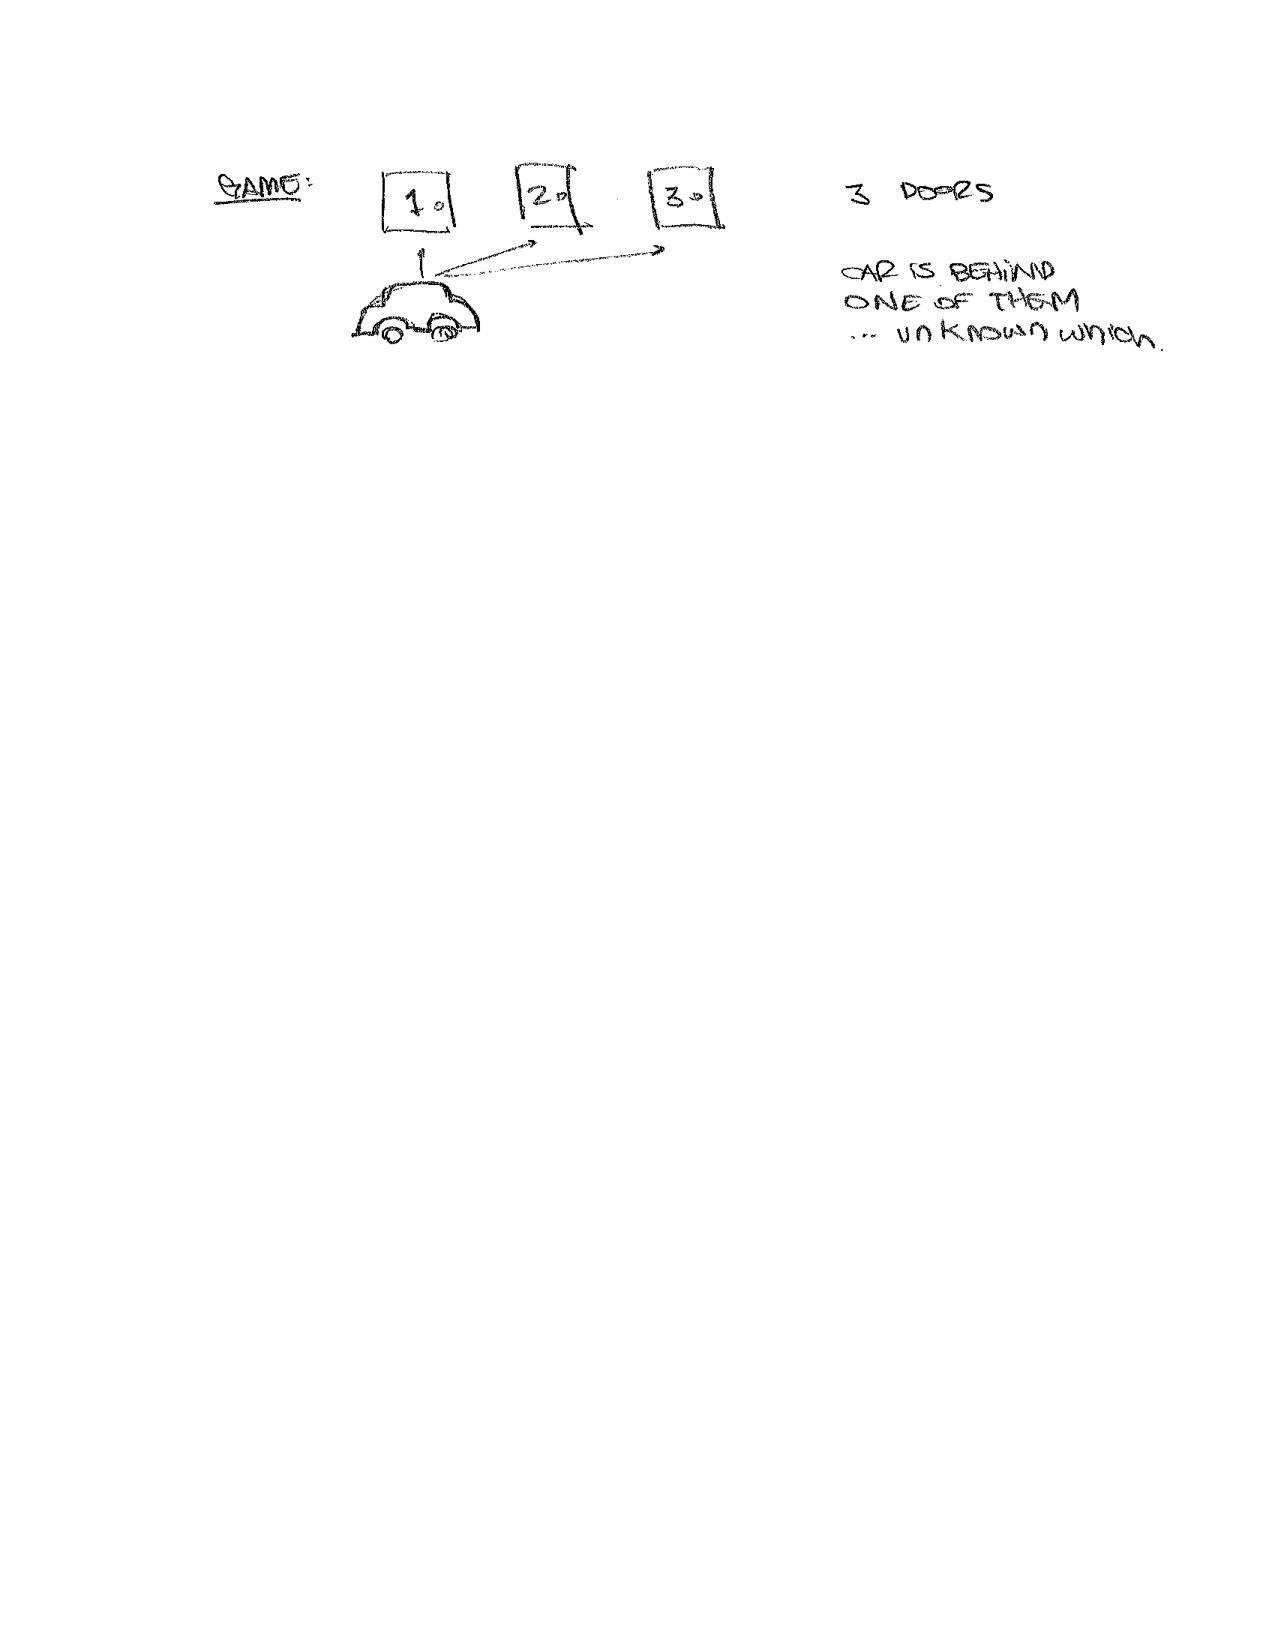
\includegraphics[width=.7\textwidth]{figures/Monty_01.pdf}
\end{center}
The contestant picks one of the three doors. Rather than opening that door immediately, the host offers a twist. The host---who has perfect knowledge of which door has the car---selects a second door and opens it, revealing no prize. 
\begin{center}
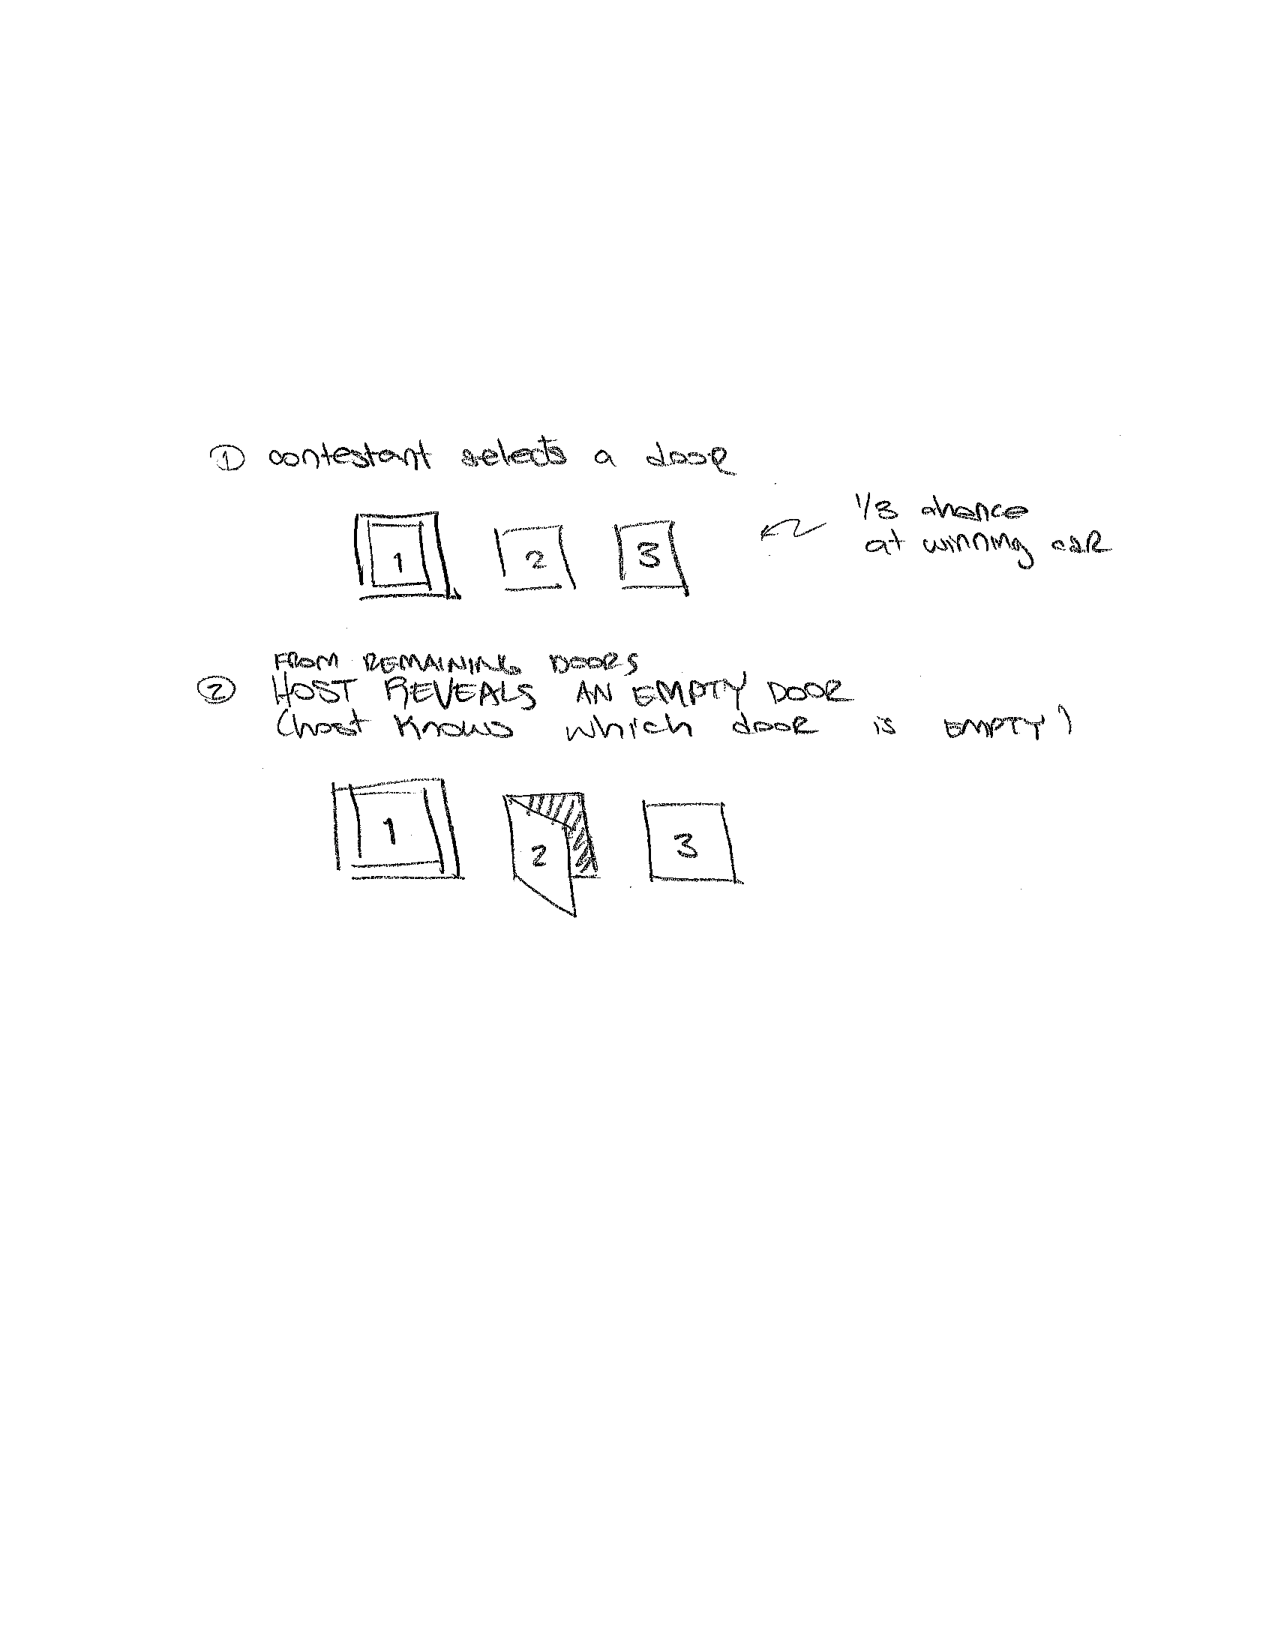
\includegraphics[width=.7\textwidth]{figures/Monty_02.pdf}
\end{center}
The host then offers the contestant the opportunity to either open the door they have currently selected, or to change their mind and instead select the remaining unopened door. There are now two perspectives, leading to what may appear to be a paradox:
\begin{enumerate}
	\item The contents of doors are equally unknown to the contestant, so it does not matter whether or not the contestant swaps choices.
	\item At the beginning of the game, the choice of a door has a 1/3 chance of winning the car. After the host has revealed one empty door, the choice if 1/2. If the contestant does not swap doors, then they are effectively locking in their 1-in-3 chance from the beginning of the game. Thus it makes sense for the contestant to swap choices since this locks in a 1-in-2 chance.
\end{enumerate}
Bayes theorem gives us the tools to quantify this puzzle. For concreteness, assume that the contestant initially chooses door 1, the host reveals door 2 to be empty, and then the host offers door 3. We would like to compare the following quantities
\begin{itemize}
	\item $P(1\,|\,\text{open}~2)$, the probability that the car is behind door 1 after the host has revealed that it is not in door 2. That is, the probability that the contestant wins by \emph{not} swapping doors.
	\item $P(3\,|\,\text{open}~2)$, the probability that the car is behind door 3 after the host has revealed that it is not in door 2. That is, the probability that the contestant wins by \emph{swapping} doors.
\end{itemize}
We are \emph{not} comparing either of these to $P(1)$, the probability that the car is behind door 1 \emph{prior} to any information about the other doors. In order to calculate the above conditional probabilities, we invoke Bayes' theorem.
\begin{align}
	P(1\,|\,\text{open}~2) = \frac{P(\text{open}~2\,|\,1)\, P(1)}{P(\text{open}~2)} \ .
\end{align}
The prior probability is $P(1)=1/3$. The first factor in the numerator is the probability that the host opens door 2 \emph{assuming} that the car is actually behind door 1. If the contestant were correct with their initial guess, then the host could have opened door 2 or 3. Thus $P(\text{open}~2\,|\,1)=1/2$. The denominator is the probability that the host would have revealed door 2 without any constraint from the contestant. Because there are two choices of empty doors, this is  $P(\text{open}~2)=1/2$. As a result, the \emph{posterior} probability is
\begin{align}
	P(1\,|\,\text{open}~2) = \frac{1}{3} \ .
\end{align}
We interpret this as follows: if the contestant does not to switch doors and remains with door 1, the odds of them winning is 1-in-3. 

What if the contestant switches? Bayes tells us
\begin{align}
	P(3\,|\,\text{open}~2) = \frac{P(\text{open}~2\,|\,3)\, P(3)}{P(\text{open}~2)} \ .
\end{align}
The denominator is unchanged. Similarly, the prior probability $P(3)=P(1)=1/3$ is unchanged. However, $P(\text{open}~2\,|\,3)$ is rather different. This is the probability that the host opens door 2 given that the actual car is behind door 3. However, what is not well conveyed in our notation---but nonetheless is true when applying Bayes' theorem---is that the host's choice is constrained by the fact that they \emph{cannot} reveal either (1) the door that the contestant has selected, or (2) the door that actually has the car. In this conditional probability, the host has no choice: they \emph{must} select door 2 since the contestant has selected door 1 and the car is behind door 3. This means that $P(\text{open}~2\,|\,3) = 1$. With that in mind, we have
\begin{align}
	P(3\,|\,\text{open}~2) = \frac{2}{3} \ .
\end{align}
Of course, we already knew this had to be true since conservation of probability tells us that $P(1\,|\,\text{open}~2)+P(3\,|\,\text{open}~2)=1$.

\subsection{Information Entropy}

In statistical mechanics we have a notion of \textbf{entropy},
\begin{align}
	S = -\sum_i p_i \ln p_i \ ,
\end{align}
where $p_i$ is the probability of a configuration. We have assumed $k_B=1$, a kind of `natural units' for statistical mechanics. 

\begin{example}
\textbf{Microcanonical ensemble}. For the microcanonical ensemble, all $N$ possible states have equal probability so that $p_i = 1/N$. Then the entropy is $S = -N^{-1}\sum_i\ln N^{-1} = \ln N$, which simply measure the logarithm of the number of microstates. 
\end{example}

There is a closely related idea in information theory called \textbf{information entropy} or Shannon entropy,
\begin{align}
	H = -\sim_i p_i \log_2 p_i \ ,
\end{align}
where the binary base tells you that we are counting bits of information. The Shannon entropy measures the information in a configuration. A bit is corresponds to reducing the uncertainty by a factor of two. Over the last ten years, information entropy has found its way into physics, so it is worth taking a moment to familiarize ourselves with the idea. 

There is an excellent pedagogical example by Aur\'elien G\'eron. Suppose we live somewhere where the weather has a 50\% chance each of being sunny or rainy. If the weather report says it will definitely rain tomorrow, then it has reduced the uncertainty relative to the baseline scenario by one bit: you went from two equal possibilities to one possibility. 

Similarly, if there were four equal probabilities (sun, rain, fog, snow), then a definite forecast reduces the uncertainty from 4 equally possible states to one. In other words, the forecast provides $2$ bits of information to reduce the number of possibilities by $1/2^2$. If there were eight equally possible weather possibilities, then a definite forecast provides $4$ bits of information that reduces the number of possibilities by $1/2^4$. 

The uncertainty reduction from a specification of a state is the inverse of the probability of that state. We find a convenient definition: when there are $N$ equal probabilities for all possible states, the \textbf{number of bits} encoded in a message that specifies a state is simply $\log_2 N$.

Of course, the weather analogy so far is pretty silly for us since we live in Riverside. In a climate slightly closer to Riverside, the odds of rain are only 25\% and the odds of a sunny day are 75\%. You expect it to be sunny tomorrow. This means that if the national weather service tells us that it will actually rain tomorrow, it has conveyed \emph{more information} than the case of equal probabilities. In other words, the information in a message can be interpreted as the degree of \emph{surprise} relative to the expected probability distribution. The uncertainty reduction coming from a rainy forecast is
\begin{align}
	\frac{1}{P(\text{rain})} = \frac{1}{25\%} = 4 \ .
\end{align}
The rainy forecast reduces our uncertainty by $4=2^2$, or $\log_2 4=-\log_2 P(\text{rain})=2$ bits. Alternatively, if the forecast is sunny, then we are not particularly impressed. That is what we expected. The number of bits is $-\log_2P(\text{sun}) = -\log_2(75\%) \approx 0.4$.

This gives a useful general definition: \textbf{information entropy} is the expected number of bits given a statement of the state:
\begin{align}
	H(p) = \langle -\log_2 p_i \rangle = \sum_i (-\log_2 p_i)\, p_i \ .
\end{align}
This explains how autocomplete algorithms work. Some letters are more frequent in English words than others. Saying that a word begins with `x' reduces the number of possible words much more than saying that the word begins with a much more common letter, like `e'.

\flip{To do: cross entropy, KL divergence.}


